\chapter{INTRODUCTION}
\label{chap-one}

%% Following sections are examples... not required
%--
\section{Definitions}
\label{sec:def}
%--

Define common terms used throughout the dissertation... 

E.g. African Easterly Waves (AEWs) are waves in the atmosphere over Africa of wavelength ...

%--
\section{Motivations}
\label{sec:mot}
%--

Motivations for studying topic

Figure useful to motivations

\begin{figure}[htp]
\centering
\includegraphics[width=\textwidth]{Chapter-1/figs/Damage.png}
\caption{Caption...}
\label{fig:damage}
\end{figure}

Figure with trim and clip
\begin{figure}[htp]
\centering
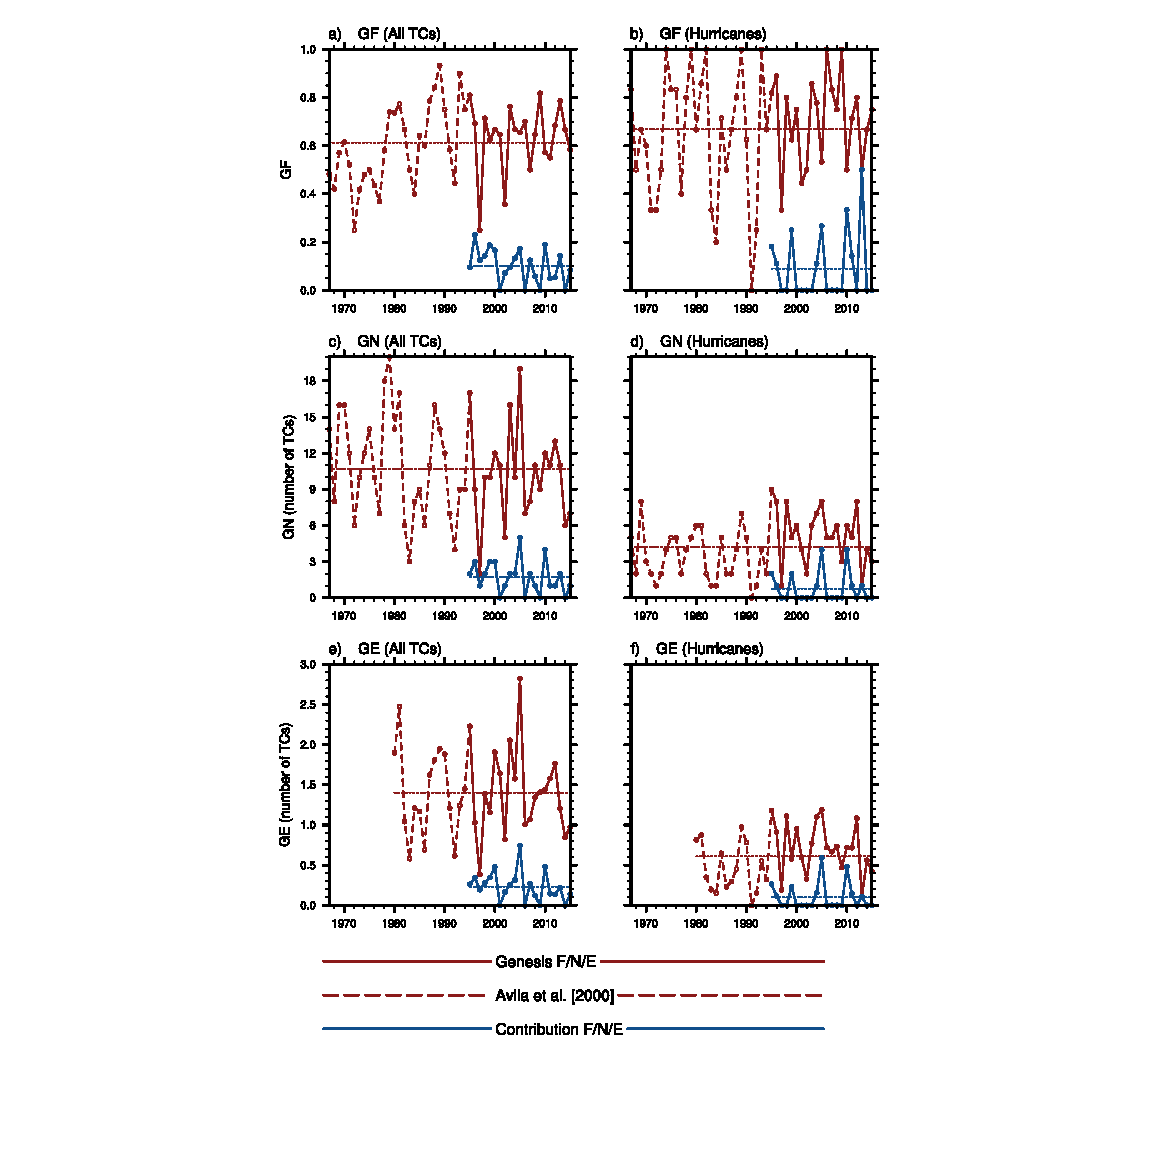
\includegraphics[trim={4cm 8.5cm 3cm 0cm},clip,width=\textwidth]{Chapter-1/figs/gfgnge_vs_year.eps}
\caption{Caption...}
\label{fig:gfgn}
\end{figure}

%--
\section{Background}
\label{sec:back}
%--

Background literature on topic

Possible citation in parentheses \citep{kiladis2006three} 

Possible citation in parentheses with text before or after also in parentheses \citep[e.g. ][ Figure 1]{kiladis2006three} 

Citation in text \citet{tomassini2017interaction}

%----------
\section{Open Questions and Theories}
\label{sec:que}
%----------

In this section I will present the open questions on the problem I am investigating. 

\subsection{Influence of AEWs on Convection}
\label{sec:QTaew-conv}

Background on theories

In summary we will attempt to address the following questions with regard to ...:
\begin{enumerate}
\item Question 1?
\item Question 2?
\item Question 3?
\end{enumerate}
